\chapter{Noarr Library}\label{chap:noarr}

Our work on abstractions for high-performance computing introduced layout-agnostic and traversal-agnostic abstractions that enable separation of concerns between data representation, data traversal, and algorithm implementation. We have developed two main abstractions: Noarr~\cite{vsmelko2022astute,klepl2024pure,klepl2024abstractions,klepl2025layout} and Cellato~\cite{brabec2025cellato} as experimental testbeds for exploring and showcasing these ideas. % TODO: resolve the disbalance between Noarr and Cellato

\section{Noarr Structures}

Noarr structures, introduced in our initial work~\cite{vsmelko2022astute}, are the fundamental abstraction in the Noarr library used to model multi-dimensional data layouts according to the principles of layout agnosticism.

\begin{figure}[ht]
  \centering
  \begin{subfigure}{.3\linewidth}
    \centering
    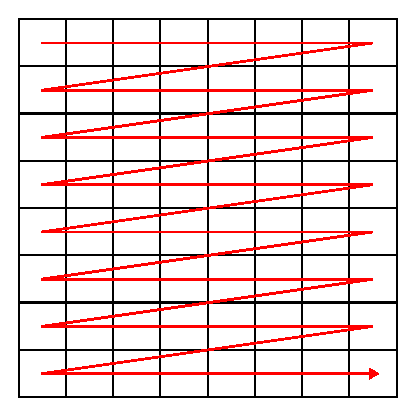
\includegraphics[width=.9\linewidth]{img/row-major.eps}
    \caption{Row-major layout}%
    \label{fig:row-major}
  \end{subfigure}%
  \hfill%
  \begin{subfigure}{.3\linewidth}
    \centering
    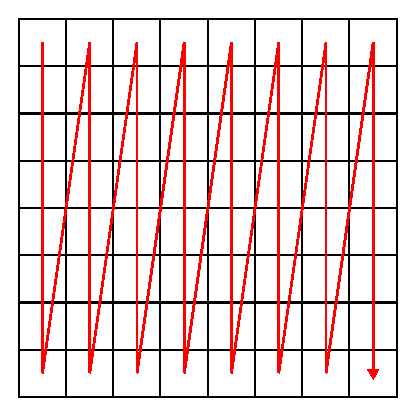
\includegraphics[width=.9\linewidth]{img/column-major.eps}
    \caption{Column-major layout}%
    \label{fig:column-major}
  \end{subfigure}%
  \hfill%
  \begin{subfigure}{.3\linewidth}
    \centering
    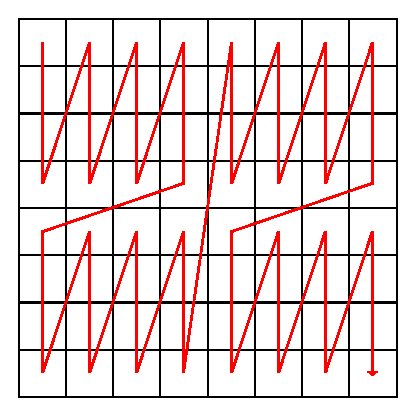
\includegraphics[width=.9\linewidth]{img/tiled.eps}
    \caption{Tiled layout}%
    \label{fig:tiled}
  \end{subfigure}%
  \caption{Examples of different data layouts for a 2D array.}%
  \label{fig:data-layouts}
\end{figure}

\Cref{fig:data-layouts} illustrates multiple data layouts for a 2D array, including row-major, column-major, and tiled layouts. Noarr structures are designed to be flexible and extensible to support the shown and many other layouts, as well as their transformations (the tiled layout at \cref{fig:tiled} is a transformation of the column-major layout at \cref{fig:column-major}).

\Cref{fig:row-major} and \cref{fig:column-major} have the same logical structure (a 2D array) but different physical layouts in memory. We call the design of an algorithm \emph{layout-agnostic} if an involved data structure can be in any of the layouts sharing the same logical structure (having the same index space) without requiring changes to the algorithm implementation. Noarr structures are designed to have this property without sacrificing performance.

A Noarr structure is, at its core, a compile-time interpreted description that maps a multi-dimensional index space to a linear memory layout --- this makes them related to abstractions such as \texttt{std::mdspan}~\cite{trott2022mdspan}, Kokkos Views~\cite{trott2021kokkos}, or CuTe Layouts~\cite{thakkar2023cutlass}. To enable layout agnosticism, each dimension of its index space is associated with a \emph{dimension name}. This allows the algorithm to access the data using semantically meaningful index names instead of relying on the order of dimensions in the layout.

A simple example of a layout-agnostic algorithm for matrix multiplication using Noarr structures is shown in \cref{lst:layout-agnostic-matmul}. For this example, we assume three data structures defined using Noarr: \texttt{matrixA}, \texttt{matrixB}, and \texttt{matrixC}, which represent the two input matrices and the output matrix, respectively. What makes the algorithm layout-agnostic is that it indexes the data structures using points in the index space (e.g., \texttt{idx<'i', 'j', 'k'>(i, j, k)}) instead of relying on the order (and presence) of individual dimensions in the layout of each data structure --- for example, \texttt{matrixA} is indexed using the dimensions \texttt{'i'}, and \texttt{'k'}, while \texttt{matrixB} is indexed using the dimensions \texttt{'k'} and \texttt{'j'}, and the order typically matters in non-agnostic algorithms. This contrasts a typical non-agnostic implementation of matrix multiplication in \cpp shown in \cref{lst:layout-non-agnostic-matmul}, where the algorithm relies on the order of dimensions in the layout (e.g., \texttt{i * N + j} assumes a specific layout of the data in memory) and thus is not layout-agnostic. Since the layout-agnostic algorithm in \cref{lst:layout-agnostic-matmul} does not use any explicit offset calculations, it makes the approach simpler and cleaner, avoiding many opportunities for mistakes in the indexing logic (e.g., using \texttt{i * N + k} instead of \texttt{i * K + k} in the non-agnostic version).

\begin{lstlisting}[language=C++, caption={A layout-agnostic matrix multiplication algorithm using Noarr structures.}, label={lst:layout-agnostic-matmul}]
auto matrixC = /*...*/;
auto matrixA = /*...*/;
auto matrixB = /*...*/;

for (size_t i = 0; i < (matrixC | get_length<'i'>()); ++i) {
  for (size_t j = 0; j < (matrixC | get_length<'j'>()); ++j) {
    matrixC[idx<'i', 'j'>(i, j)] = 0;
    for (size_t k = 0; k < (matrixA | get_length<'k'>()); ++k) {
      auto point = idx<'i', 'j', 'k'>(i, j, k);
      matrixC[point] += matrixA[point] * matrixB[point];
    }
  }
}
\end{lstlisting}


\begin{lstlisting}[language=C++, caption={A layout-non-agnostic matrix multiplication algorithm in \cpp.}, label={lst:layout-non-agnostic-matmul}]
float* matrixC = /*...*/;
float* matrixA = /*...*/;
float* matrixB = /*...*/;

for (size_t i = 0; i < M; ++i) {
  for (size_t j = 0; j < N; ++j) {
    matrixC[i*N + j] = 0;
    for (size_t k = 0; k < K; ++k) {
      matrixC[i*N + j] += matrixA[i*K + k] * matrixB[k*N + j];
    }
  }
}
\end{lstlisting}

% In this simple example, the differences seem to exchange the complexity of the indexing logic (which is not quite complex in this case) for a more verbose and less familiar syntax of the layout-agnostic version. However, if, for example, a tiling is applied to the computation (a typical optimization for matrix multiplication), the indexing logic in the non-agnostic version becomes more complex and error-prone, while the layout-agnostic version remains unchanged.

The example in \cref{lst:layout-agnostic-matmul} also shows another important aspect of Noarr structures --- they allow for querying other properties of the data layout, such as the length of a dimension (e.g., \lstinline{matrixC | get_length<'i'>()}) or the total size of the data structure (e.g., \lstinline{matrixC | get_size()}). This barely scratches the surface of the capabilities of Noarr structures, but it illustrates yet another important aspect of the layout-agnostic approach. If an algorithm is parametrized by an input data structure, it should be able to infer the important properties of the data layout from the data structure itself, without requiring additional parameters or assumptions about the layout.

\section{Noarr Traversals}
